%%%%%%%%%%%%%%%%%%%%%%%%%%%%%%%%%%%%%%%%%
% FRI Data Science_report LaTeX Template
% Version 1.0 (28/1/2020)
% 
% Jure Demšar (jure.demsar@fri.uni-lj.si)
%
% Based on MicromouseSymp article template by:
% Mathias Legrand (legrand.mathias@gmail.com) 
% With extensive modifications by:
% Antonio Valente (antonio.luis.valente@gmail.com)
%
% License:
% CC BY-NC-SA 3.0 (http://creativecommons.org/licenses/by-nc-sa/3.0/)
%
%%%%%%%%%%%%%%%%%%%%%%%%%%%%%%%%%%%%%%%%%


%----------------------------------------------------------------------------------------
%	PACKAGES AND OTHER DOCUMENT CONFIGURATIONS
%----------------------------------------------------------------------------------------
\documentclass[fleqn,moreauthors,10pt]{ds_report}
\usepackage[english]{babel}

\graphicspath{{fig/}}




%----------------------------------------------------------------------------------------
%	ARTICLE INFORMATION
%----------------------------------------------------------------------------------------

% Header
\JournalInfo{FRI Natural language processing course 2024}

% Interim or final report
\Archive{Project report} 
%\Archive{Final report} 

% Article title
\PaperTitle{LLM Prompt Strategies for Commonsense-Reasoning Tasks} 

% Authors (student competitors) and their info
\Authors{Tesa Robič, Tim Dolenc and Matjaž Bevc}

% Advisors
\affiliation{\textit{Advisors: Aleš Žagar}}

% Keywords
\Keywords{Promp Engineering, Mistral Instruct, NLP, LLM, Commonsense-Reasoning}
\newcommand{\keywordname}{Keywords}


%----------------------------------------------------------------------------------------
%	ABSTRACT
%----------------------------------------------------------------------------------------

\Abstract{
This project evaluates different prompting strategies for commonsense reasoning tasks using the Mistral-7B-Instruct model. We explored methods such as Zero-Shot Chain of Thought (CoT), Plan-and-Solve (PS, PS+), and our Auto FewShot approach.
}

%----------------------------------------------------------------------------------------

\begin{document}

% Makes all text pages the same height
\flushbottom 

% Print the title and abstract box
\maketitle 

% Removes page numbering from the first page
\thispagestyle{empty} 

%----------------------------------------------------------------------------------------
%	ARTICLE CONTENTS
%----------------------------------------------------------------------------------------

\section*{Introduction}

    In this project we will research, compare and evaluate different prompt strategies for commonsense reasoning tasks used in Large Language Models (LLM). LLMs are really good at understanding and generating text. But when it comes to understanding common sense (the things we know about the world without being told), they need help. So, researchers are trying out different ways to give these models hints or instructions, called prompts. There are many different prompt strategies like Chain Of Thought (CoT), In-Context Learning (ICL), plan-and-solve techniques, Tree Of Thought, Retrieval augmentation (RAG) and more. In the next chapter, we introduce different already existing solutions that we consider using for this project. Another strategy that we develop is Auto FewShot explained later in chapter Methods.\cite{Prompt} 
	


%------------------------------------------------
\section*{Existing solutions and Realated Work}

\subsection*{Chain-of-Thought (CoT) prompting}

Chain-of-thought prompting enables large language models to tackle complex arithmetic, commonsense, and symbolic reasoning tasks. CoT prompting involves providing intermediate reasoning steps to guide the model’s responses, which can be facilitated through simple prompts such as “Let’s think step by step” or through a series of manual demonstrations, each composed of a question and a reasoning chain that leads to an answer. \cite{Prompt} 

    \begin{figure}[ht]\centering
    	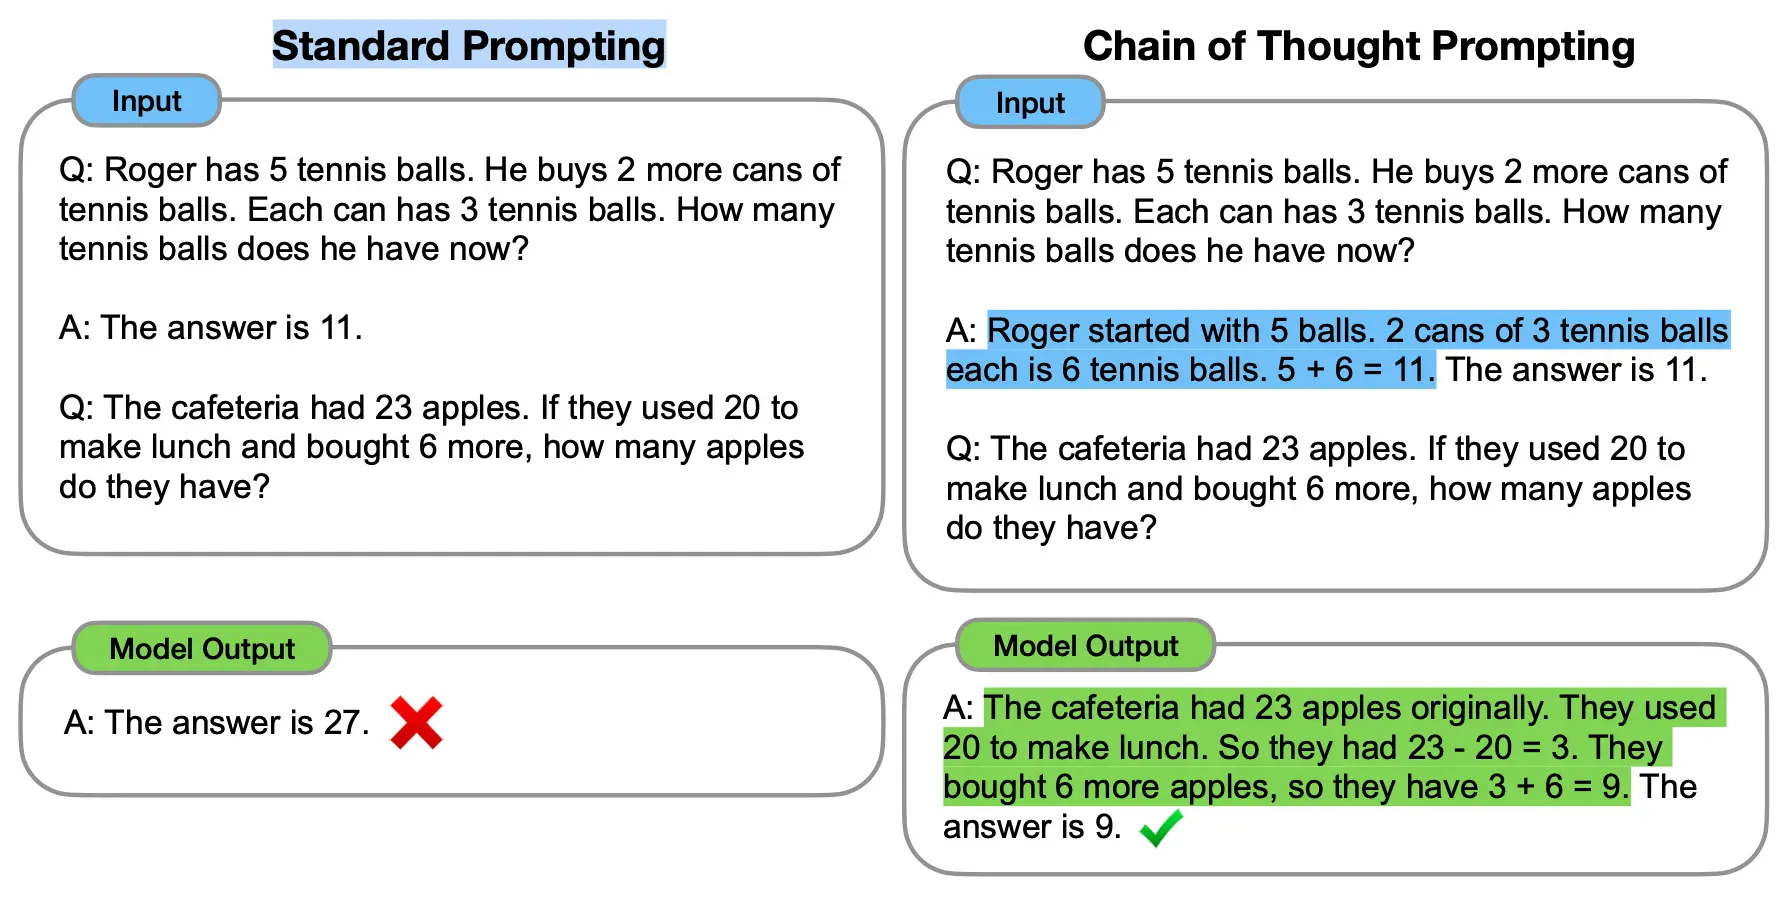
\includegraphics[width=\linewidth]{cot.png}
    	\caption{\textbf{CoT Prompting.} An illustration of standard LLM prompting on the left, and chain-of-thought prompting on the right.}
    	\label{fig:column}
    \end{figure}
\bigskip
\bigskip
\bigskip
\bigskip
\bigskip\bigskip
\bigskip\bigskip
\bigskip\bigskip
\bigskip
Some benefits of CoT promting:
\begin{itemize}
    \item \textbf{Improved accuracy}: With clear reasoning steps, the LLM is less likely to make mistakes or jump to illogical conclusions. This is especially helpful for tasks with multi-step logic or complex reasoning requirements.
    \item \textbf{Transparency:} CoT prompts make the reasoning process more transparent, allowing us to understand how the LLM arrived at its answer. This is crucial for building trust and identifying potential bias or errors.
    \item \textbf{Better performance on complex tasks:} CoT is particularly effective for tasks that require multi-step reasoning, logical deduction or \textit{common-sense} application. These are areas where past LLMs often struggled.
    \item \textbf{Adaptability}: The technique can be used for various tasks, from solving math problems and interpreting data to summarizing text and even creative writing.
    \item \textbf{Precision-Guided Reasoning:} By providing a clear path, CoT reduces the risk of LLMs stumbling into erroneous conclusions or leaps of illogical faith. Multi-step tasks and convoluted reasoning problems, once impenetrable to LLMs, become navigable landscapes with CoT at the helm. \cite{cot} 

\end{itemize}


Limitations of CoT prompting:
\begin{itemize}
    \item \textbf{Manual effort:} Creating effective CoT prompts requires understanding the problem and designing the reasoning steps yourself. This can be time-consuming and complex for intricate tasks.
    \item \textbf{Model size:} CoT seems to be more effective for larger LLMs with stronger reasoning capabilities. Smaller models might struggle to follow the prompts or generate their own reasoning chains.
    \item \textbf{Prompt bias:} Like any other prompting technique, CoT can be susceptible to biased prompts that lead the LLM to incorrect conclusions. Careful design and testing are crucial.
    \item \textbf{Bias Blind Spots:} Just like any prompt, CoT is susceptible to biased information. Careful design and thorough testing are crucial to ensure the LLM doesn’t follow a misleading path
    \item \textbf{Crafting the Path:} Building effective CoT prompts requires understanding the problem’s intricacies and formulating a clear, logical chain of reasoning. This can be demanding, especially for complex tasks. \cite{cot} 

\end{itemize}
\subsubsection*{Zero Shot CoT}
 Zero Shot Chain of Thought (Zero shot CoT) prompting is a follow up to CoT prompting, which introduces an incredibly simple zero shot prompt. After each question we append the words "Let's think step by step."  or a similar text, to extract step-by-step reasoning. After that LLMs are able to generate a chain of thought that answers the question. \cite{Zero} 

\subsection*{Plan-and-Solve (PS) prompting}
With Zero-shot CoT, there are three pitfalls: calculation errors, missing-reasoning-step errors and semantic understanding errors. 

The first two pitfalls can be addressed with Plan-and-Solve prompting (PS and PS+).
\newline

Plan-and-Solve prompting consists of two components: devising a plan to divide the task into small subtasks and carrying out the subtasks according to the plan. While Zero-Shot CoT appends the phrase \textit{"Let's think step by step"} to the prompt, PS appends \textit{"Let’s first understand theproblem and devise a plan to solve the problem. Then, let’s carry out the plan and solve the problem step by step." }
\newline

Extending the prompt with additional phrases gets us to PS+. For example, in case of complex arithmetic calculations, these phrases can be added:
\begin{itemize}
    \item \textit{"pay attention to calculation"}
    \item \textit{"extract relevant variables and their corresponding numerals"}
    \item \textit{"calculate intermediate results"}
    \item \textit{"pay attention to commonsense reasoning"}
\end{itemize}

This requests precise calculations from the LLM, tells it to not leave out relevant variables and enhances its ability to generate reasoning steps.
\newline

There are two main limitations of PS and PS+:
\begin{itemize}
    \item It takes effort to design the prompt to generate correct reasoning steps.
    \item PS(+) can address calculation errors and missing reasoning-step errors, but it cannot help against semantic misunderstanding errors. \cite{ps}
\end{itemize}

\subsection*{Few-Shot Prompting}

In Few-Shot Prompting, the model is provided with a small set of examples within the prompt itself. These examples are selected to demonstrate the task or the type of response desired. By analyzing these examples, the LLM learns the context and structure of the task, allowing it to apply this understanding to new, similar problems. Few-Shot Prompting is akin to In-Context Learning (ICL), but instead of providing analogies, it furnishes the prompt with concrete examples followed by the LLM's desired answers. 

For instance, consider the following examples:
\begin{itemize}
    \item Example 1: "Emma left her keys in the freezer. Why? - Emma was carrying a lot of things and absent-mindedly put her keys in the freezer."
    \item Example 2: "Mike found his phone in the bathroom cabinet. Why? - Mike was multi-tasking, cleaning the bathroom while talking on the phone, and he left it there accidentally."
\end{itemize}

Now, when the LLM is presented with the target question about John's coffee cup, it has context from these examples on how to approach and solve the problem:

\textit{Target Question with Few-Shot Learning Applied}:
\begin{quote}
    "John found his coffee cup in the refrigerator. Why was it there?"
\end{quote}
Based on the learning from the examples, the LLM might reason in the following manner:
\begin{itemize}
    \item Similar to Emma, who absent-mindedly left her keys in the freezer while being preoccupied with carrying multiple items, it is plausible that John was also engaged in multitasking.
    \item Drawing a parallel with Mike's situation, where his attention was divided, leading to him leaving his phone in the bathroom, John might have been similarly distracted.
    \item Consequently, it is reasonable to infer that John could have placed his coffee cup in the refrigerator during a moment of absent-mindedness or distraction, akin to the scenarios described in the examples.
\end{itemize}



\section*{Methods}

For this research we choose Mistral-7B-Instruct-v0.2 LLM, which is an instruct fine-tuned version of the Mistral-7B-v0.2. All previously described strategies and one described in this chapter were applied to this model using two datasets. \cite{mistral} 


\subsubsection*{Auto Few shot}


    
    We implemented an automatic few-shot learning approach to enhance the main question-answering process. This method identifies the three most similar questions from the dataset (based on cosine similarity) and incorporates these examples, along with their answers, to provide context for the main question. Here's how it works:
    
    \begin{quote}
        \textbf{Main question} Given the question 'What do people aim to do at work?' and the following choices: A: complete job, B: learn from each other, C: kill animals, D: wear hats, E: talk to each other, which one is correct? Answer only with one of the following A, B, C, D, or E. \textbf{[End of main question]}
    \end{quote}
    
    is expanded with examples in the following way:
    
    \begin{quote}
        \textbf{Introduction} You will see examples and a main question. Please provide the answer to the main question based on these examples. Your response can only include one character: A, B, C, D, or E. \textbf{[End of introduction]}
    \end{quote}
    
    \begin{quote}
        \textbf{Example question} Given the question 'A person would join a trade school for finding information related to what?' and the following choices: A: ulcers, B: degree, C: understanding of, D: gaining knowledge, E: happiness, which one is correct? Answer only with one of the following A, B, C, D, or E. \textbf{[End of example question]} \\
        \textbf{Answer} D \textbf{[End of answer]}
    \end{quote}
    
    \begin{quote}
        \textbf{Example question} Given the question 'Where is known to be a wealth of information?' and the following choices: A: park, B: internet, C: meeting, D: library, E: book, which one is correct? Answer only with one of the following A, B, C, D, or E. \textbf{[End of example question]} \\
        \textbf{Answer} D \textbf{[End of answer]}
    \end{quote}
    
    \begin{quote}
        \textbf{Example question} Given the question 'What is another name for the color of the fur of a dog with light-colored fur?' and the following choices: A: fair, B: basket, C: dog hair, D: game, E: sun, which one is correct? Answer only with one of the following A, B, C, D, or E. \textbf{[End of example question]} \\
        \textbf{Answer} A \textbf{[End of answer]}
    \end{quote}
    
    \begin{quote}
        \textbf{Main question} Given the question 'What do people aim to do at work?' and the following choices: A: complete job, B: learn from each other, C: kill animals, D: wear hats, E: talk to each other, which one is correct? Answer only with one of the following A, B, C, D, or E. \textbf{[End of main question]}
    \end{quote}

\subsubsection*{Finding Similar Questions Based on Cosine Similarity}

The example questions are found by calculating the cosine similarity between the TF-IDF vectors of the questions with the following steps:

\begin{enumerate}
    \item Extract the text of the questions from the dataset.
    \item Vectorize the questions using TF-IDF (Term Frequency-Inverse Document Frequency).
    \item Compute the cosine similarity between the vectorized main question and all other questions in the dataset.
    \item Select the top N questions with the highest similarity scores.
\end{enumerate}

\subsection*{Datasets}
We utilized two benchmark datasets, CommonsenseQA and CommonGen, to evaluate our model's performance. CommonsenseQA provided us with a robust framework for multi-question answering, while CommonGen allowed us to generate responses in natural language, thus offering a comprehensive assessment of the model's capabilities across different tasks.
\subsubsection*{CommonsenseQA}
The CommonsenseQA is a dataset for commonsense question answering task. The dataset consists of 12,247 questions with 5 choices each. For our project we used validation set containing 1221 examples. \cite{talmor-etal-2019-commonsenseqa}
\subsubsection*{CommonGen}
CommonGen is constructed through a combination of crowd-sourced and existing caption corpora, consists of 79k commonsense descriptions over 35k unique concept-sets. For our project we used validation set containing 4018 examples. Answers are generated in natural language, containing all three concepts. \cite{lin-etal-2020-commongen}

\subsection*{Implementation}
We structured our code into two main components, one utilizing multiple-answer questions CommonsenseQA dataset and another generative dataset CommonGen.
\newline
For each dataset we formatted questions to fit the models requirements. 
We tested all the examples from the validation split from both datasets using each of the prompting strategies we described earlier. This thorough approach helped us see how well each strategy worked and how the model performed in different situations. After collecting all the results we evaluated model's performance using different approaches described in next chapter.




%------------------------------------------------

\section*{Results}
\subsection*{CommonsenseQA evaluation}
We used accuracy as the evaluation metric for multi-question answers using the CommonsenseQA dataset. 
The accuracy of the model is defined as:

\begin{equation}
\text{Accuracy} = \frac{\text{Number of Correct Predictions}}{\text{Total Number of Questions}}
\end{equation}

This metric provides a straightforward measure of the model's performance in predicting the correct answers. Here is a table containing accuracy percentage for different strategies:

\begin{table}[h!]
\centering
\begin{tabular}{@{}ll@{}}
\toprule
\textbf{Strategy} & \textbf{Accuracy [\%]} \\ \midrule
no strategy & 53.89 \\
Zeroshot CoT & 53.40 \\
Plan and solve & 55.45 \\
Plan and solve + & 56.59 \\
Auto few shot  & 55.55. \\ \bottomrule
\end{tabular}
\caption{Accuracy comparison}
\label{tab:example}
\end{table}

We got the highest accuracy using PS+ strategy which we crafted special for commonsense reasoning tasks. 
To every prompt, we added the following: "Let's first prepare relevant information and make a plan. Then, let's answer the question step by step (pay attention to commonsense and logical coherence)." This addition aims to guide the model in systematically approaching and solving commonsense reasoning tasks. 


\subsection*{CommonGen evaluation}
\subsubsection*{Automatic Metrics}
To evaluate how well the Mistral Instruct model performs, we used several well-known metrics to measure the quality and accuracy of its outputs. These metrics are BLEU, ROUGE, METEOR, and BERTScore, and each gives us a different way to look at the model's performance:

\begin{itemize}
    \item BLEU: Measures how much the generated text matches the reference text in terms of exact words and phrases.
\end{itemize}
\begin{itemize}
    \item ROUGE: Checks how well the generated text captures the key ideas and phrases from the reference text.
\end{itemize}
\begin{itemize}
    \item METEOR: Considers synonyms and variations, focusing on the overall meaning and alignment of the text.
\end{itemize}
\begin{itemize}
    \item BERTScore leverages the contextual embeddings from BERT (Bidirectional Encoder Representations from Transformers) to evaluate text similarity. It measures the semantic similarity between the generated and reference texts at the token level, offering a robust assessment of the contextual and semantic alignment of the outputs.
\end{itemize}

Before running evaluation script we have done some pre-processing, including extraction. 

Our result are shown in table, containing average scores from different metrics:
\begin{table}[h!]
\centering

\begin{tabular}{lcccc}
\toprule
\textbf{Strategy} & \textbf{BLEU} & \textbf{ROUGE} & \textbf{METEOR} & \textbf{BERT} \\
\midrule
Baseline & 0.05 & 0.40 & 0.36 & 0.89 \\
ZeroShot CoT & 0.05 & 0.37 & 0.34 & 0.89 \\
PS & 0.06 & 0.42 & 0.37 & 0.90 \\
PS+ & 0.05 & 0.35 & 0.31 & 0.89 \\
auto FewShot & X & X & X & X \\
\bottomrule
\end{tabular}
\caption{Evaluation Scores for Different Prompting Strategies}
\label{tab:scores}
\end{table}
\newline
The evaluation metrics BLEU, ROUGE, and METEOR are relatively low, while BERTScore is high across the different strategies. This discrepancy can be explained by the nature of these metrics and the characteristics of the generated sentences.

\textbf{BLEU}, \textbf{ROUGE}, and \textbf{METEOR} primarily measure word overlap and the exact match of n-grams between the generated text and the reference text. These metrics are sensitive to differences in word choice and phrasing. Consequently, they tend to give lower scores when there are variations in the specific words used, even if the overall meaning of the sentences is similar.

\textbf{BERTScore}, on the other hand, evaluates the semantic similarity between the generated text and the reference text by comparing their embeddings. This metric is less sensitive to exact word matches and more focused on the overall meaning of the sentences. As a result, BERTScore can remain high even when there are differences in word choice and phrasing, as long as the generated text conveys a similar meaning to the reference text.

In our experiments, the sentences generated using the given concepts are semantically similar to the reference sentences, but they often use different words and phrasing. This leads to lower scores in BLEU, ROUGE, and METEOR, which rely on exact matches, while still achieving high BERT-Score, which captures the semantic similarity.





\subsubsection*{Human evaluation}
We choose this criteria for evaluating common sense reasoning tasks:

\begin{itemize}
    \item Common Sense Understanding: Does the text demonstrate an understanding of everyday situations and common sense knowledge?
\end{itemize}

\begin{itemize}
    \item Logical Consistency: Are the conclusions drawn logically consistent with the given information and common sense?
\end{itemize}

\begin{itemize}
    \item Realism: Does the text describe situations and events realistically and believably?
\end{itemize}

\begin{itemize}
    \item Inference & Problem-solving: Does the text make reasonable inferences and effectively solve the problem presented?
\end{itemize}

\begin{itemize}
    \item Intuitiveness & Novelty: Is the reasoning process intuitive and understandable, providing unique insights beyond the prompt?
\end{itemize}

Each of the three group members evaluated ten random examples and gave 1 - 5 grade for each criteria, 1 meaning poor and 5 meaning excellent. After that we computed the average score of our rating for different strategies. Here is the representations of our evaluation:
    \begin{figure}[ht]\centering
    	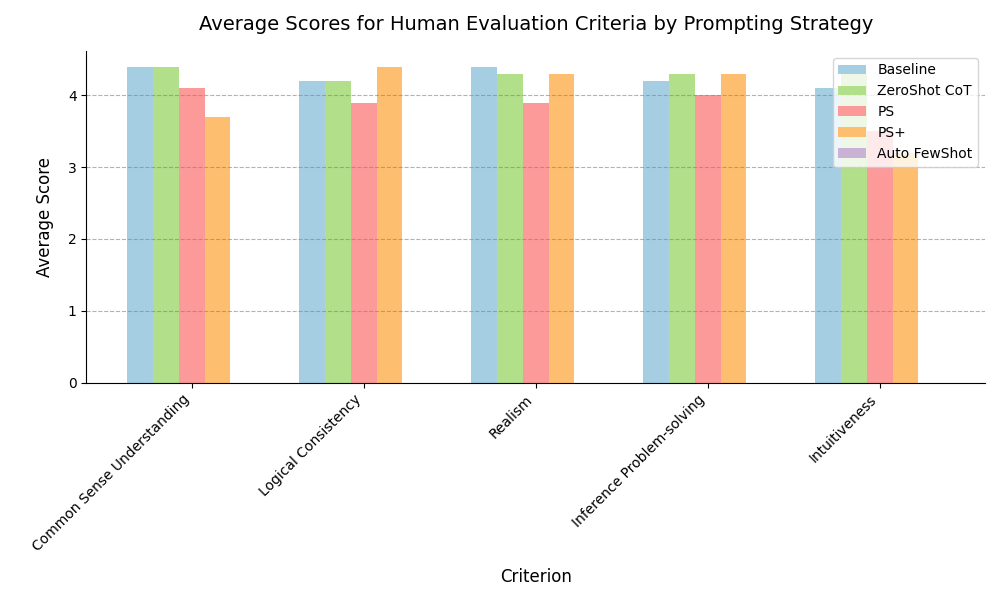
\includegraphics[width=\linewidth]{report/fig/average_scores_prompting_strategies_minimalistic.png}
    	\caption{\textbf{Human Evaluation} Representation of our rating on different strategies}
    	\label{fig:column}
    \end{figure}






%------------------------------------------------

\section*{Discussion}
Our evaluation of various prompting strategies for commonsense reasoning tasks using the Mistral-7B-Instruct model showed that while Plan-and-Solve (PS+) had the highest accuracy, the differences from the baseline were not significant. This suggests that while structured reasoning prompts provide some improvement, their overall impact may be limited. Traditional metrics like BLEU, ROUGE, and METEOR showed low scores, though BERTScore indicated good semantic coherence. Human evaluation stressed the importance of common sense understanding and logical consistency, but overall, the strategies did not significantly outperform the baseline, indicating the need for further refinement.

%------------------------------------------------

\section*{Acknowledgments}

We would like to thank our advisor Aleš Žagar who guided us through this project and helped us overcome various problems.


%----------------------------------------------------------------------------------------
%	REFERENCE LIST
%----------------------------------------------------------------------------------------
\bibliographystyle{unsrt}
\bibliography{report}


\end{document}